\newpage

\section{It is also possible to generate a beta distribution using gamma distributions. A gamma distribution $Ga(\alpha, \beta)$ is defined by the density function $f(x|\alpha, \beta) := \frac{\beta^\alpha}{\Gamma(\alpha)} x^{\alpha - 1} e^{-\beta x} \mathbb{I}_{[0, +\infty[}(x) \text{for } \alpha, \beta > 0$.} \label{sec:5}

% -------------------------------------------------------------------------------------------------

\subsection*{(a) Show formally that if $Y_1 \sim Ga(\alpha, 1)$ and $Y_2 \sim Ga(\beta, 1)$ then $X = \frac{Y_1}{Y_1 + Y_2} \sim Be(\alpha, \beta)$.}

Let $Y_1 \sim \text{Ga}(\alpha, 1)$ and $Y_2 \sim \text{Ga}(\beta, 1)$, where the gamma density function is defined as:
\begin{equation}
f_{Y_1}(y_1 \mid \alpha, 1) = \frac{1}{\Gamma(\alpha)} y_1^{\alpha - 1} e^{-y_1}, \quad y_1 > 0,
\end{equation}
\begin{equation}
f_{Y_2}(y_2 \mid \beta, 1) = \frac{1}{\Gamma(\beta)} y_2^{\beta - 1} e^{-y_2}, \quad y_2 > 0.
\end{equation}

Since \(Y_1\) and \(Y_2\) are independent, their joint density is the product:
\begin{equation}
f_{Y_1,Y_2}(y_1, y_2 \mid \alpha, \beta) = \frac{1}{\Gamma(\alpha)\Gamma(\beta)} y_1^{\alpha - 1} y_2^{\beta - 1} e^{-(y_1 + y_2)}, \quad y_1, y_2 > 0.
\end{equation}

Define the new variable that $X = \frac{Y_1}{Y_1 + Y_2}$, $T = Y_1 + Y_2$. This transformation maps $(Y_1, Y_2) \mapsto (X, T)$, with inverse of $Y_1 = X T$, $Y_2 = (1 - X) T$. To derive the joint density of $(X, T)$, we compute the Jacobian determinant:
\[
J = \left| \frac{\partial (Y_1, Y_2)}{\partial (X, T)} \right| = 
\begin{vmatrix}
\frac{\partial Y_1}{\partial X} & \frac{\partial Y_1}{\partial T} \\
\frac{\partial Y_2}{\partial X} & \frac{\partial Y_2}{\partial T}
\end{vmatrix}
=
\begin{vmatrix}
T & X \\
- T & 1 - X
\end{vmatrix}
= T(1 - X) + T X = T
\]

Now, the joint density becomes:
\begin{align}
f_{X,T}(x, t \mid \alpha, \beta) &= f_{Y_1, Y_2}(x t, (1 - x)t \mid \alpha, \beta) \cdot |J| \\
% &= f_{Y_1}(x t) \cdot f_{Y_2}((1 - x)t) \cdot t \\
&= \frac{1}{\Gamma(\alpha) \Gamma(\beta)} (x t)^{\alpha - 1} e^{-x t} \cdot ((1 - x) t)^{\beta - 1} e^{-(1 - x) t} \cdot t \\
&= \frac{1}{\Gamma(\alpha)\Gamma(\beta)} x^{\alpha - 1} (1 - x)^{\beta - 1} t^{\alpha + \beta - 1} e^{-t}
\end{align}

for \(x \in (0,1)\), \(t > 0\).


Using Eq. (\ref{eq:1-12}), stating that $B(\alpha, \beta) = \frac{\Gamma(\alpha)\Gamma(\beta)}{\Gamma(\alpha + \beta)}$, the joint density is rewritten as:
\begin{equation}
f_{X,T}(x, t \mid \alpha, \beta) = \underbrace{\frac{1}{B(\alpha, \beta)} x^{\alpha - 1} (1 - x)^{\beta - 1}}_{f_X(x \mid \alpha, \beta)} \cdot \underbrace{\frac{1}{\Gamma(\alpha + \beta)} t^{\alpha + \beta - 1} e^{-t}}_{f_T(t \mid \alpha, \beta)}.
\end{equation}

Since the joint density factorizes into a product of marginal densities, \(X\) and \(T\) are independent. Furthermore, their marginal distributions are:
\[
X \sim \text{Be}(\alpha, \beta), \quad x \in (0,1),
\]
\[
T \sim \text{Ga}(\alpha + \beta, 1), \quad t > 0.
\]


% ---

% Assuming the independence between $Y_1$ and $Y_2$, the joint probability density function is given by:
% \[
% f_{Y_1, Y_2}(y_1, y_2) = f_{Y_1}(y_1)f_{Y_2}(y_2) = \frac{y_1^{\alpha - 1}e^{-y_1}}{\Gamma(\alpha)} \cdot \frac{y_2^{\beta - 1}e^{-y_2}}{\Gamma(\beta)}
% \]

% Considering the following change of variables $X = \frac{Y_1}{Y_1 + Y_2}$ and $Z = Y_1 + Y_2$, we have $Y_1 = XZ$ and $Y_2 = Z - XZ$. The Jacobian determinant of the transformation is equal to $Z$. The joint density of $X$ and $Z$ is:
% \[
% f_{X,Z}(x,z) = \frac{(xz)^{\alpha - 1}e^{-(xz)} \cdot (z - xz)^{\beta - 1}e^{-(z - xz)}}{\Gamma(\alpha)\Gamma(\beta)} \cdot z
% \]

% \[
% f_{X,Z}(x,z) = \frac{z^{\alpha + \beta - 1}e^{-z}x^{\alpha - 1}(1 - x)^{\beta - 1}}{\Gamma(\alpha)\Gamma(\beta)}
% \]

% \[
% f_{X,Z}(x,z) = \frac{1}{\Gamma(\alpha + \beta)} z^{\alpha + \beta - 1}e^{-z} \cdot \frac{\Gamma(\alpha + \beta)}{\Gamma(\alpha)\Gamma(\beta)} x^{\alpha - 1}(1 - x)^{\beta - 1}
% \]

% We can see that the first part of the product is a Gamma distribution $Z \sim \text{Ga}(\alpha + \beta, 1)$ and the second part is a beta distribution $X \sim \text{Be}(\alpha, \beta)$ (This corresponds to what we wanted to show).


% -------------------------------------------------------------------------------------------------

\newpage
\subsection*{(b) Use this relation to construct an algorithm to generate a beta random variable and simulate 15,000 values from a $Be(3, 9)$.}

Based on the result in part (a), we can simulate a Beta-distributed random variable using two independent Gamma random variables. Specifically, if $Y_1 \sim \text{Gamma}(\alpha, 1)$ and $Y_2 \sim \text{Gamma}(\beta, 1)$, then the ratio
\[
X = \frac{Y_1}{Y_1 + Y_2}
\]
follows a $\text{Be}(\alpha, \beta)$ distribution.

\subsubsection*{Simulation and results}

To simulate 15,000 samples from $\text{Be}(3, 9)$, we use the following algorithm:

\begin{enumerate}
    \item Generate $Y_1 \sim \text{Gamma}(3, 1)$ and $Y_2 \sim \text{Gamma}(9, 1)$.
    \item Compute $X = \frac{Y_1}{Y_1 + Y_2}$.
    \item Repeat this process 15,000 times to obtain a sample of size 15,000.
\end{enumerate}

\begin{figure}[H]
    \centering
    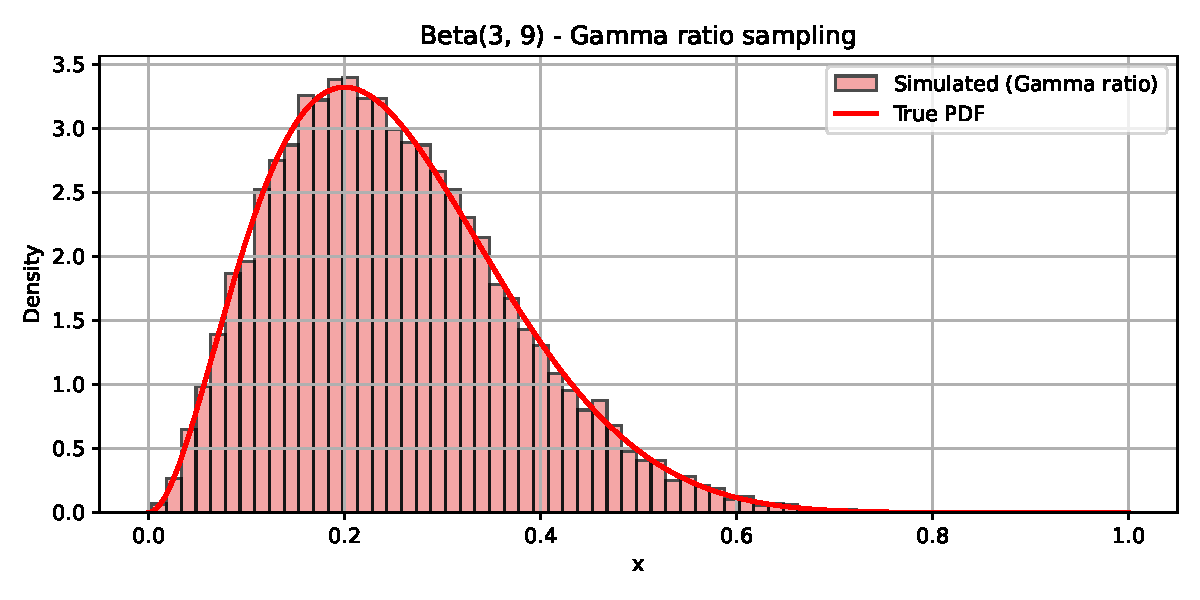
\includegraphics[width=0.7\textwidth]{resources/figures/q5-beta_gamma_ratio_sampling.pdf}
    \noskipcaption{Histogram of 15,000 samples from $\text{Be}(3, 9)$ using the Gamma ratio method (red), with the true density overlaid.}
    \label{fig:q5-beta_gamma}
\end{figure}

As shown in Figure~\ref{fig:q5-beta_gamma}, the empirical distribution obtained from the Gamma ratio sampling aligns very well with the theoretical probability density function of the $\text{Be}(3, 9)$ distribution. This confirms the correctness and efficiency of the method.

% \subsection*{Conclusion}

% The Gamma ratio method provides an elegant and general approach to generating Beta-distributed random variables for arbitrary positive values of $\alpha$ and $\beta$. Unlike the transformation method from Question 4, this approach is not limited to integer parameters and is widely applicable in practical simulations.





% \section{It is also possible to generate a beta distribution using gamma distributions. A gamma distribution $Ga(\alpha, \beta)$ is defined by the density function $f(x|\alpha, \beta) := \frac{\beta^\alpha}{\Gamma(\alpha)} x^{\alpha - 1} e^{-\beta x} \mathbb{I}_{[0, +\infty[}(x) \text{for } \alpha, \beta > 0$.}

% \subsection*{(a) Show formally that if $Y_1 \sim Ga(\alpha, 1)$ and $Y_2 \sim Ga(\beta, 1)$ then $X = \frac{Y_1}{Y_1 + Y_2} \sim Be(\alpha, \beta)$.}

% \subsection*{(b) Use this relation to construct an algorithm to generate a beta random variable and simulate 15,000 values from a $Be(3, 9)$.}